% !TEX root = ../Main.tex

Since the isolation and characterisation of
Graphene in 2004 by Andre Geim and
Konstantin Novoselov, scientists have marvelled over the physical properties and potential
application of Graphene. Being a relatively new material, many aspects and ideas are being
investigated and researched at all times. Graphene yield extreme tensile strength as well as
extreme electric conductivity, yet its structure is fairly simple. Graphene consists solely of
carbon atoms thus making it easy to simulate using specialised software, since carbon atoms are greatly understood in terms of chemical
bonding.
As graphene is a very versatile material the possibilities for research in simulation environments are virtually limitless.
Therefore it is basically possible to make experiments limited only by imagination, in order
to discover new properties and possible applications of graphene. This saves resources
before entering the lab, where the simulated reality is tested.

In this rapport we will simulate and analyse the properties of nanomembranes. In the article "Visualizing the Motion of Graphene Nanodrums"\cite{Davidovikj2016}, from which \cref{Motivation} originate, nanomembranes on a microscale are simulated and experimentally tested. The article describes how phonons travel through these membranes. The results of the work in the article and many others suggests that the simulated phonon models holds true for systems on the micrometer scale when tested in the lab. We will examine if this same phenomenons are found at the nano-scale. To do this we start by considering a ideal system of just one sheet of carbon atoms. By simulating this ideal system in a virtual environment we will analyse the vibrational modes, and frequencies in said modes. By simulating various sizes of membranes, we will examine how scaleable our analysis turns out to be.
We will employ the software Atomistic ToolKit (ATK)\cite{QuantumWise} to carry out these simulations. The
software will enable prompt setup of relevant structures with variying parameters.
Afterwards in order to make a more realistic scenario we will investigate whether you can create the same membrane effects if you take a graphene layer and put it on top of a substrate with different sized holes, a nanomesh, to form a two layer membrane.
The nanomesh can be fabricated as done in the paper "Graphene nanomesh"\cite{Bai2010} where nanomeshes are created with holes of about 20 nm diameter, depicted in \cref{dootdoot}
It is expected possible to create such a nanomesh at the
size of few tens of nanometers at DTU Nanotech with Block-copolymer lithography or TEM
structuring of a substrate.
We will simulate and analyse these two layer membranes and then compare them to the idealised membranes.
We assume that the nanomembranes will have similar properties as the bigger holes for \cref{Motivation}.
The purpose of this project is to
simulate phonons in the nanomembrane and find the optimal conditions for producing
phonons in the terahertz spectrum.
% \begin{figure}
%     \centering
%     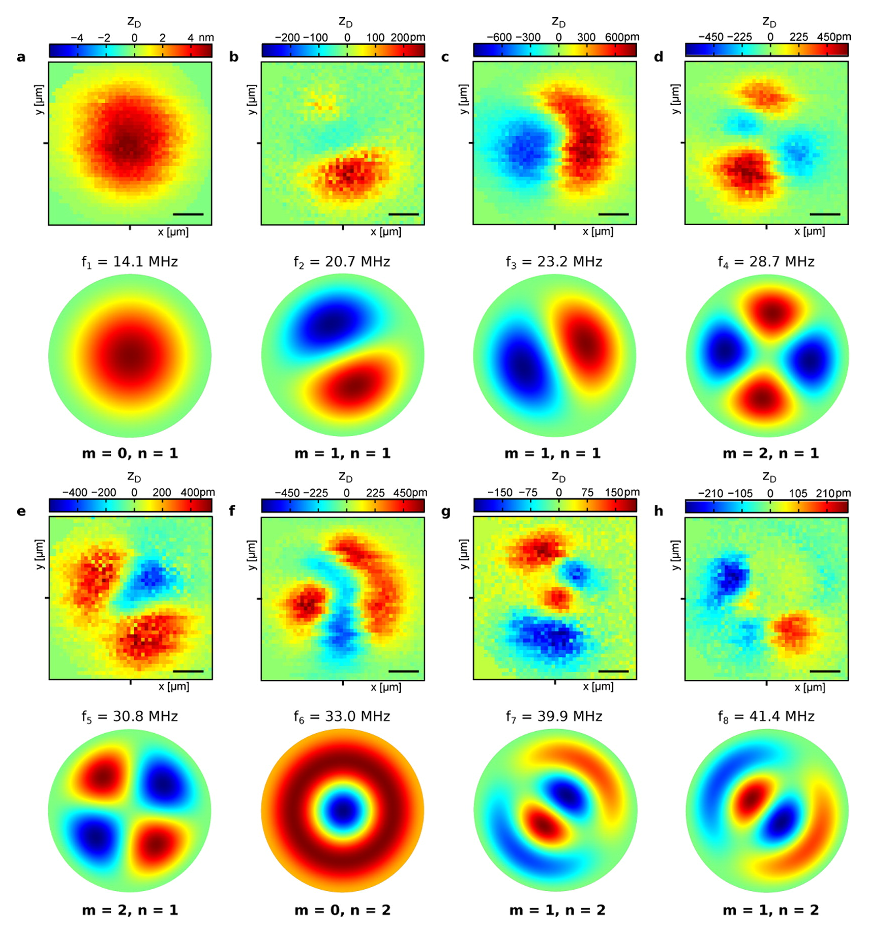
\includegraphics[width=0.5\textwidth]{Figures/motivation.eps}
%     \caption{Visualizing resonant motion. (a–h) Top, experimental data; bottom, finite-element calculation. The modes predicted by the calculation are indexed by (m,n). Panels b and c show that the nanodrum hosts a split degenerate (1,1) mode, while also the (2,1) mode is split, as is shown in panels d and e. The displacement profile measured in panel f resembles a (0,2) mode, which is distorted due to an imperfection as discussed in the main text. Panels g and h reveal a degenerate (1,2) mode. Scale bars: 1 $\mathrm{\mu m}$.\cite{Davidovikj2016}}
%     \label{Motivation}
% \end{figure}
% \begin{figure}
%     \centering
%     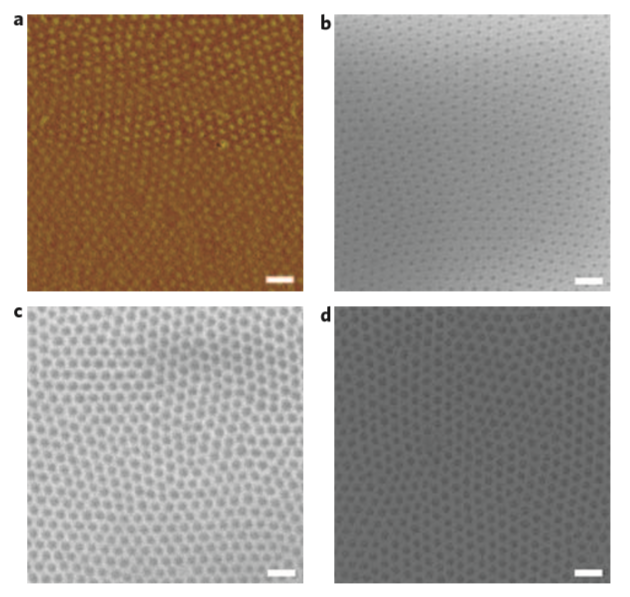
\includegraphics[width=0.5\textwidth]{Figures/jaminkan.PNG}
%     \caption{Images illustrating the steps of the nanomesh fabrication process. a, AFM phase contrast image of the annealed block-copolymer film on graphene, showing hexagonal-packed PMMA domains in the PS matrix. b, SEM image of a porous PS film obtained by selectively removing the PMMA domains. c, SEM image of the $\mathrm{SiO}_x$ nanomesh mask after reactive ion etching with the PS mask. d, SEM image of a GNM structure after removing the top $\mathrm{SiO}_x$ mesh mask. Scale bars, 100 nm.\cite{Bai2010}}
%     \label{dootdoot}
% \end{figure}